\section{SIR SpectroSim Runner}\label{sec:sir_runner}

Link to the gitlab repository

\begin{center}
\hypertarget{url:sir_runner_gitlab}{\url{https://gitlab.euclid-sgs.uk/lpagan01/SIR_SpectroSim_Runner}}
\end{center}

\subsection{Overview}

The code \verb+SIR_SpectroSim_Runner+ was born with the aim to automate the running of TIPS in a customized way, allowing the user to choose in an \emph{easy} way:

\begin{itemize}
\item the instrumental effects to be included in the simulation;
\item the input catalogs and spectra of the astronomical sources to be simulated;
\item the set of input XML files for TIPS.
\end{itemize}

The software requires a \verb+JSON+ input file, described in \secref{subsec:input_JSON} with all these information, and takes care of setting up the workspace and managing the workflow for running TIPS which is illustrated in \figref{fig:TIPS_workflow}. After some time it became necessary also to have a way to launch also the SIR data reduction Pipeline on the results of the simulation, and therefore this feature was added to the code.\\
\textbf{IMPORTANT}: up to now the code works with \verb+SIM_TIPS_Simulator+ version \verb+4.6.8+ and \verb+SIR_Pipeline+ version \verb+1.0.0+.

\subsection{Input JSON file}\label{subsec:input_JSON}
This file is structured as a nested python dictionary. It is important \textbf{to not modify any of the dictionary keys}. You can find a template of this JSON file into the \verb+SIR_SpectroSim_Runner+ repository, looking into

\begin{center}
\verb+SIR_SpectroSim_Runner/SimulationManager/auxdir/json_templates/testsim.json+
\end{center}

Here we provide a description of each entry of the file.

\paragraph{\texttt{SimulationID}} A string with the ID of the simulation, which will be used to name the directory of the simulation.

\paragraph{\texttt{processing\_steps}} a dictionary of boolean switches for the detector effects.

\paragraph{\texttt{keyval\_params}} another dictionary of boolean switches for other instrumental effects, which are not included in the previous entry. This distinction is made by TIPS itself, so it has been adopted for simplicity.

\paragraph{\texttt{flags}} a dictionary of lists, representing the flags to pass to each of the three main TIPS programs. Here the only physically relevant flag is the \verb+no_simspc+ flag for the \verb+EuclidNisSplit+ program. This flag forces TIPS to use the input spectra provided by the user in the \verb+SpectraFitsFile+, since by default the code generates the spectra of the sources automatically according to template Spectral Energy Densities (SEDs).

\paragraph{\texttt{catalogs}} These are the catalogs and spectra fits files described in \secref{subsubsec:catalogs_spectra_fits}, to be written in the TU XML file.

\paragraph{\texttt{source\_dir}} The directory containing all the input files. Refer to \secref{subsec:source_directory} for a description of the structure of this directory.

\paragraph{\texttt{input\_xml\_files}} The paths, relative to the \verb+source_dir+, of the TIPS XML input files to be used in the simulation.

\paragraph{\texttt{grism\_sequence}} A list of four pairs, one per dither, where the i-th pair stores the grism to be used for the i-th along with the tilt, expressed in degrees.

\paragraph{\texttt{dithering\_offsets}} A list of four pairs, one per dither, each storing the coordinate offsets $\Delta$RA and $\Delta$DEC of each dither, w.r.t. the telescope pointing coordinates specified in the \verb+DpdNisInputConfiguration+ XML file. 

\paragraph{\texttt{SpectralOrders}} A string containing the spectral orders to be simulated, represented by capital letters delimited with whitespaces.

\subsection{Input files directory structure}\label{subsec:source_directory}

\begin{figure}
    \centering
    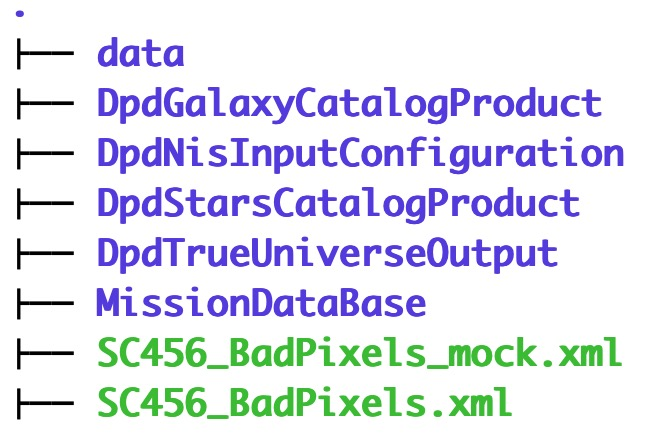
\includegraphics[scale=0.2]{figures/source_dir_structure.jpg}
    \caption{Structure of the source directory.}
    \label{fig:source_dir_structure}
\end{figure}

The \verb+source_dir+ entry of the JSON file points to the directory storing all the input XML and FITS files for running TIPS. This directory must have the structure depicted in \figref{fig:source_dir_structure}. Each of the \verb+Dpd*+ directories must contain its corresponding DataProduct XML file, with the \verb+MissionDataBase+ directory containing the MDB XML files. The \verb+data+ directory must contain all the input FITS files. I suggest to look at the following path on ZEFIRO INFN cluster

\begin{center}
\verb+/gpfs/ddn/euclid/SIR_spectroscopic_simulations/workdir+
\end{center}

where you can find all the data that are needed to run the simulations. Simply do an \verb+rsync+ from there to a directory of your local machine, and you are done.
\textbf{N.B.:} the size of this directory is about 23 GB.

\subsection{Installation}
The installation of the code is divided in three steps

\begin{enumerate}
\item Clone the repository from the gitlab \hyperlink{url:sir_runner_gitlab}{link} into your \verb+$HOME/Work/Projects+ directory;
\item Enter the directory \verb+$HOME/Work/Projects/SIR_SpectroSim_Runner+ and select the branch of the code you want to use. I suggest to use a tagged version, for example \verb+TIPS_4.6.8_SIR_1.0.0+;
\item install the code by running the command \verb+make install+, thus rendering it available for usage with \verb+E-Run+.
\end{enumerate}

\subsection{Main program usage}
The main program of \verb+SIR_SpectroSim_Runner+ is named \verb+launch_simsir+, and can be run with \verb+E-Run+ as shown in \secref{sec:framework}

\begin{center}
\verb+E-Run SIR_SpectroSim_Runner launch_simsir <parameters>+
\end{center}

In order to get the help message showing the available parameters type

\begin{center}
\verb+E-Run SIR_SpectroSim_Runner launch_simsir -h+
\end{center}

I always suggest to call this script specifying the path to a log file through the parameter \verb+--log-file /path/to/logfile+.\\
There are three main modes for this program:

\begin{itemize}
\item Only SIM: run only TIPS simulation;
\item Only SIR: run only SIR Pipeline on an existing simulation;
\item SIM + SIR: run TIPS and then SIR Pipeline on the simulation produced by TIPS.
\end{itemize}

Here the description of each of the three usages.

\paragraph{Only SIM}
In order to trigger this mode you have to provide the flag parameter \verb+--only_sim+. The only mandatory input in this case is the path to the input JSON file described in \secref{subsec:input_JSON}. However, if you want to use a specific version of TIPS, say \verb+4.6.8+, I also suggest to specify it through the \verb+--tips_version+ parameter. If this parameter is not passed, then the code will try to run a local installation of \verb+SIM_TIPS_Simulator+ into \verb+$HOME/Work/Projects+. An example call in this case is

\begin{verbatim}
E-Run SIR_SpectroSimRunner launch_simsir 
--only_sim --json_input /path/to/json --tips_version 4.6.8
--save_sim_midfiles --nframes 1
--log-file /path/to/logfile
\end{verbatim}

\paragraph{Only SIR}
In order to trigger this mode you have to provide the flag parameter \verb+--only_sir+. In this case the only mandatory input is the path to the simulation directory produced by the code in the \verb+only_sim+ mode. You must provide this path through the parameter \verb+--sir_workdir+. If you want to provide the version of SIR Pipeline you can do it through the parameter \verb+--sir_pipeline_version+. If this parameter is not provided, the code will try to us a local installed version of \verb+SIR_Pipeline+ looking for it into \verb+$HOME/Work/Projects+.
An example call in this case is

\begin{verbatim}
E-Run SIR_SpectroSimRunner launch_simsir 
--only_sir --sir_workdir /path/to/sir/workdir
--sir_pipeline_version 1.0.0  --nframes 1
--log-file /path/to/logfile
\end{verbatim}

\paragraph{SIM + SIR}
This mode is the default, and it is triggered without passing any particular flag. It goes without saying that in this case the code will run a simulation TIPS and then the SIR Pipeline on the resulting simulation. The mandatory input in this case is the same as in the \verb+only_sim+ mode, i.e. the path to the JSON input file. An example call is

\begin{verbatim}
E-Run SIR_SpectroSim_Runner launch_simsir 
--json_input /path/to/json
--tips_version 4.6.8 --sir_pipeline_version 1.0.0
 --nframes 1 --save_sim_midfiles --log-file /path/to/logfile
\end{verbatim}

As in the previous cases, if one or both of \verb+--tips_version+ and \verb+--sir_pipeline_version+ parameters are not passed, the code will try to run local installed versions of TIPS and SIR Pipeline which happen to be into \verb+$HOME/Work/Projects+.

\subsection{Simulation directory structure}

\begin{figure}
\centering
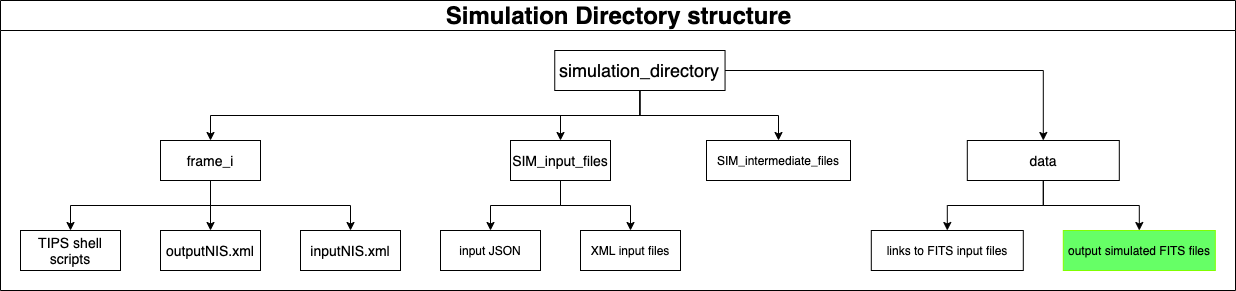
\includegraphics[scale=0.35]{figures/TIPS_usage-sir_runner_dir_structure.png}
\caption{Schema of directory structure for a simulation generated with the \texttt{SIR\_SpectroSim\_Runner} code.}
\label{fig:sim_dir_tree}
\end{figure}

The directory created for the simulation will have the following naming pattern

\begin{verbatim}
<SimulationID>_YY-mm-ddTHH-MM-SS
\end{verbatim}

where \verb+<SimulationID>+ is the entry specified in the JSON input file, and the rest is the date-time string, with 4-digits year format. Under this directory there will be as many sub-directories named \verb+frame_?+ as it is specified via the \verb+--nframes+ parameter of the main program \verb+launch_simsir+. Essentially a frame corresponds to a dither of the telescope. Each of these \verb+frame+ directories contains an XML file named \verb+outputNIS_frame_?.xml+ which contains the name of the output FITS file for that given dither. The output FITS frame is located into the sub-directory \verb+data+ colored by orange in \figref{fig:sim_dir_tree}.